\documentclass[UTF8]{ctexart}
\usepackage{graphicx} % Required for inserting images
\usepackage{amsmath,amssymb,amsthm}
\usepackage{physics}
\usepackage{graphicx,float}
\graphicspath{{images/}}
\usepackage[none]{hyphenat}
\usepackage{blindtext}
\usepackage{parskip}
\usepackage[letterpaper,top=3cm, left= 3cm,bottom=3cm]{geometry}
\usepackage{subcaption}
\numberwithin{equation}{section}

\begin{document}
\section{洛伦兹变换}
在本题中,你将重走爱因斯坦的道路,推导狭义相对论中的时空变换(又称洛伦兹变换),并由此推导一些有意思的结论。\textbf{以下所有推导均在惯性系中进行}。
\subsection{准备工作}
\begin{enumerate}
    \item 在正式推导开始前,请简单阐述洛伦兹变换和牛顿力学中伽利略变换的区别
    \item 人类是如何意识到伽利略变换失效的?
\end{enumerate}
\subsection{伽利略变换}
在推导洛伦兹变换前,有必要先了解下伽利略变换。这有助于理解变换是什么,并提取些推导思路。

首先我们了解下什么是变换,考虑两个坐标系$S$系和$S'$系。伽利略变换提供了两个坐标系之间坐标$(x,y,z,t)$与$(x',y',z',t')$的转换公式。

请你推导经典理论中的伽利略变换。

提示:考虑两个坐标轴平行的参考系,在$t = 0$时,两坐标系原点重合,$S'$系相对$S$系有一个朝$+x$方向的速度$v$。

\subsection{洛伦兹变换}
推导完伽利略变换后,下面你将推导洛伦兹变换。同样考虑两个坐标轴平行的参考系,在$t = 0$时,两坐标系原点重合,$S'$系相对$S$系有一个朝$+x$方向的速度$v$。
\begin{enumerate}
    \item 洛伦兹变换中,$y$和$y'$以及$z$和$z'$的关系是什么?
    \item 下面你要建立$(x,t)$和$(x',t')$的关系,请列出$x$与$x'$和$t'$以及$t$与$x'$和$t'$的关系,你应该列出一个四元一次方程(但是方程不一定有四条),这些方程的系数是我们想求的变换系数。
    
    提示:狭义相对论认为时间和空间都是线性变化的,换句话说$S$系中的坐标增量$\Delta x$正比于$S'$系中的坐标增量$\Delta x'$,对于时间也是同理。

    \item 根据运动的相对性,$S'$系的坐标转换成$S$系也应该有类似的形式,请写出$S'$系坐标和$S$系坐标的转换式,并根据此列出两个关于转换系数的方程。
    
    提示:狭义相对论中,$x$和$t$是相互独立的。

    \item 仿照伽利略变换的思路,推导第三个关于转换系数的方程
    
    \item 现在我们列最后一个方程,根据光速不变,列出第四个关于转换系数的方程
    
    \item 列完方程后,请你解这四个方程,求出洛伦兹变换的4个系数
\end{enumerate}

\subsection{狭义相对论的应用}
本题中,你将用洛伦兹变换推导些有意思的结论
\begin{enumerate}
    \item 高速运动的尺子在相对论效应下会缩短,请证明这个结论
    \item 高速运动的钟在相对论效应下时间会变长,请证明这个结论
    \item 相对论提出的早期,有人提出了相对论效应产生的悖论。考虑一个高速运动的火车,即将穿过一个和火车静长度相同的隧道,隧道两边有可以关闭的门。在地面系中,火车会变短,故可以被关进隧道内;在火车系中,隧道会变短,故不可以被关进隧道内,一个火车不可能即被关在隧道内,又不能被关在隧道内,这就产生了悖论。请你解释这个悖论。
    \item 考虑一对双生子,一位留在地球上,一位乘坐宇宙飞船高速离开地球并在20年后返回。在地球上的双生子认为宇宙飞船上的兄弟以高速运动离开,因此他的时间过得慢,故相见时宇宙飞船上的兄弟更年轻;而宇宙飞船上的兄弟认为是地球在高速远离他,故地球上时间过得更慢,相见时地球上的兄弟应该更年轻。这个悖论又称双生子悖论,请你解释这个悖论
\end{enumerate}

\newpage
\subsection{参考答案}
\subsubsection{准备工作}
\begin{enumerate}
    \item 伽利略变换假设的是绝对的时空,换句话说时间和空间在任意一个参考系下都是不变的,而洛伦兹变换没有这种特性。
    \item 迈克耳孙-莫雷实验指出了光速在任意参考系下都是不变的,伽利略变换中,光速不变是不成立的。
\end{enumerate}

\subsubsection{伽利略变换}
\begin{figure}[H]
    \centering
    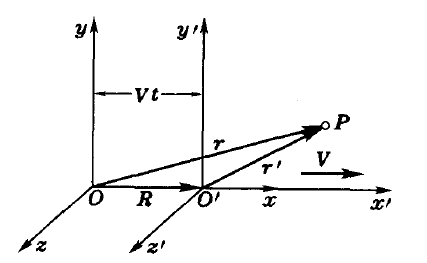
\includegraphics[width = 10cm]{Galileo.png}
    \caption{伽利略变换}
\end{figure}
很明显,$y$和$y'$坐标以及$z$和$z'$坐标是不改变的。同样,根据牛顿力学的时空观,两个坐标系下的时间坐标$t$和$t'$也相同。

因此变换的关键是求出$x$和$x'$的转换公式,不难看出$S'$系的原点在$S$系中的坐标为$vt$,因此可以得出$x' = x - vt$,至此,我们完整的推导了伽利略变换。
\[
\begin{cases}
    x' = x - vt\\
    y' = y\\
    z' = z\\
    t' = t\\
\end{cases}
\]

\newpage
\subsubsection{洛伦兹变换}
\begin{enumerate}
    \item $y' = y$,$z' = z$,因为在这两个坐标轴中没有相对运动。
    \item 
    \[
    \begin{cases}
    x = a_{11}x' + a_{12}t'\\
    t = a_{21} x' +a_{22}t'\\
    \end{cases}
    \]
    这样的假设保证了变换前后的线性时空
    \item 根据运动的相对性,$S'$相对于$S$系沿$+x$轴的方向运动等价于$S$系相对于$S'$系沿$-x'$轴运动
    \[
    \begin{cases}
    (-x')= a_{11}(-x) + a_{12}t\\
    t' = a_{21} (-x) +a_{22}t\\
    \end{cases}
    \]
    将本问求出的方程组带入上问求出的方程组的第一个式子,得到:
    \[
    (a_{11}^2 - a_{12}a_{21} - 1) x' + (a_{11}a_{12} - a_{12}a_{22})t' = 0
    \]
    时间和空间是相互独立的,不然会产生同样坐标系下不同位置时间不同的谬误,因此有
    \[
    \begin{cases}
    a_{11}^2 - a_{12}a_{21} = 1\\
    a_{11} = a_{22}\\
    \end{cases}
    \]

    \item 不难发现$S'$系的原点在$S$系中坐标为$x = vt$,带入第三问求出的方程组的第一个式子,有必要先了解下伽利略变换
    \[
    a_{12} = v a_{11}
    \]

    \item 根据光速不变原理,有
    \[
    c = \frac{x}{t} = \frac{a_{11} x' + a_{12} t'}{a_{21} x' + a_{22} t'}
    \]
    稍微化简下,有
    \[
    \frac{x'}{t'} = \frac{ca_{22} - a_{12}}{a_{11} - ca_{21}} = c
    \]
    再次化简,并带入$a_{11} = a_{22}$,得出
    \[
    a_{12} = c^2 a_{21}
    \]

    \item 先联立各个方程
    \[
    \begin{cases}
        a_{11}^2 - a_{12}a_{21} = 1\\
        a_{11} = a_{22}\\
        a_{12} = v a_{11}\\
        a_{12} = c^2 a_{21}\\
    \end{cases}
    \]
    解方程,有
    \[
    \begin{cases}
        a_{11} = \dfrac{1}{\sqrt{1-\beta^2}}\\
        a_{12} = \dfrac{v}{\sqrt{1-\beta^2}}\\
        a_{21} = \dfrac{\beta}{c\sqrt{1-\beta^2}}\\
        a_{22} = \dfrac{1}{\sqrt{1-\beta^2}}\\
    \end{cases}
    \]
    其中$\displaystyle \beta = \frac{v}{c}$,为了以后的方便,记$\displaystyle \gamma = \frac{1}{\sqrt{1-\beta^2}}$
\end{enumerate}

\subsubsection{狭义相对论的应用}
\begin{enumerate}
    \item 定义尺子长度为同一时刻测量尺子两端的坐标差。尺子相对地面观测者以$v$的速度运动,记地面系为$S$系,尺子系为$S'$系,根据之前推算的变换,有
    \[
    \Delta x' = \frac{\Delta x - v\Delta t}{\sqrt{1-\beta^2}}
    \]
    $\Delta t$为测量尺子两端坐标的时间差,$\Delta t = 0$, $\Delta x'$为尺子系中尺子长度,即尺子静长度$L_0$, $\Delta x$为地面系中尺子长度,即尺子动长度$L$,因此有
    \[
    L = L_0\sqrt{1-\beta^2}
    \]
    可以发现$\sqrt{1-\beta^2} < 0$,即运动的尺子永远比其静止的长度短

    \item 定义钟测量的时间为同一地点两个时间点测量的时间差。钟相对地面观测者以$v$的速度运动,记地面系为$S$系,钟系为$S'$系,根据洛伦兹变换,有
    \[
    \Delta t = \frac{\Delta t' + \dfrac{\beta}{c}\Delta x'}{\sqrt{1-\beta^2}}
    \]
    $\Delta x$为钟在两个测量时刻的两个坐标差,$\Delta x = 0$, $\Delta t'$为钟系中钟测量的时间长度,即静止钟测量的时间$t_0$, $\Delta t$为地面系中钟测量的时间差,即运动钟测量的时间$t$,因此有
    \[
    t = t_0 \sqrt{1-\beta^2}
    \]
    可以发现$\sqrt{1-\beta^2} < 0$,即运动的钟测量的时间永远比其静止钟测量的时间慢。

    \item 本题的关键时抓住同时的相对性,记地面系为$S$系,火车系为$S'$系,火车系中隧道关门发生的时间差为$\Delta t'$,地面系中隧道关门的时间差为$\Delta t = 0$, 二者的关系为
    \[
    \Delta t' = \frac{\Delta t - \frac{\beta}{c} \Delta x}{\sqrt{1-\beta^2}}
    \]
    其中$\Delta x$为关门发生的坐标,两坐标明显不同,即$\Delta x \neq 0$, 因此$\Delta t' \neq 0$,故在火车系中,关门发生于不同时间,不存在关不关进去的问题

    \item 宇宙飞船中的兄弟至少经历了一次加速(例如从调转速度矢量的方向,从远离地球到指向地球),因此飞船上的兄弟并不处于一个惯性参考系中,故狭义相对论在此失效,需要考虑广义相对论。
\end{enumerate}
\end{document}